\cleardoublepage

\newrefsection

\chapter{外文翻译}

本章节选了《AutoCC: Automatic discovery of Covert Channels in Time-shared Hardware》的摘要、介绍、问题背景与研究现状、方法四个部分进行翻译。
这篇文章收录于计算机体系结构顶会 56th Annual IEEE/ACM International Symposium on Microarchitecture (MICRO’23)。
我们选择这篇文章作为处理器安全漏洞形式化检测的例子。


\section*{摘要}
隐蔽信道通过观察共享硬件中的执行差异，造成了本应彼此隔离的安全域之间的信息泄露。
隐蔽信道可能出现在任何有状态的共享资源中，包括缓存、预测器和加速器。
已有工作已经识别出许多易受攻击的组件，并通过逆向工程来防御相关攻击。
然而，这种方法需要大量人工投入和推理。
随着专用硬件的“寒武纪式大爆发”，手动识别所有漏洞正变得愈发困难。

为应对这一挑战，我们提出了 AutoCC，这是一种利用形式化属性验证（Formal Property Verification，FPV）来自动发现利用进程间共享硬件的隐蔽信道的方法。
AutoCC 在寄存器传输级（Register Transfer Level，RTL）上运行，能够检查进程在一次上下文切换后留下的、任何会造成执行差异的机器状态。
一旦发现这样的差异，AutoCC 就会给出一条精确的执行轨迹，展示信息是如何被编码进机器状态并被恢复出来的。

我们在 AutoCC 生成的 FPV 测试平台上验证了我们的方案。
我们在四个开源硬件项目上对其进行了评估，其中包括两个 RISC-V 处理器和两个加速器。
在无需手写代码或定向测试的情况下，AutoCC 发现了已知的隐蔽信道（只需数分钟，而无需依赖测试驱动仿真的数小时）以及未知的隐蔽信道。
尽管 AutoCC 的主要目标是寻找隐蔽信道，我们也发现了 RTL 缺陷，这表明 AutoCC 是一种能够同时测试硬件设计安全性与可靠性的有效工具。

\section*{CCS 分类}
安全与隐私 $\rightarrow$ 侧信道分析与对策；防篡改与抗篡改设计；信息流控制；

硬件  $\rightarrow$ EDA 最佳实践。


\section*{关键词}

FPV，形式化，验证，隐蔽信道，微架构，时序信道，信息流，数据泄漏，时分，冲刷。

\section{引言}

摩尔定律的终结催生了复杂而异构的片上系统（System on Chip，SoC）设计，这些系统由多种多样的硬件模块和复杂的软件系统构成。
由于硬件模块数量庞大且其交互关系复杂，确保这些系统的安全性正变得越来越具有挑战性。
尤其是微架构隐蔽信道，它利用指令集体系结构（Instruction Set Architecture，ISA）所隐藏的硬件状态，产生了跨越安全边界的未授权信息流，对系统安全构成了重大威胁。

在基于仿真器的测试中发现异构 SoC 中的隐蔽信道，无异于大海捞针。
为了构造能够触发所有可能漏洞的测试，需要投入大量工程工作、时间和技巧。
此外，即便经验性地观察到了一个信道，也很难找到其根本原因，因为验证者往往无法直接观测到泄露信息的状态。
即使找到了原因，验证 RTL 修复是否有效也具有挑战性，因为设计改动可能会改变此前触发该问题的执行过程。

FPV 是一种很有前景的替代方案，它无需依赖测试就能以穷尽且精确的方式发现隐蔽信道。
然而，FPV 也带来了若干挑战，例如较高的学习门槛、将安全问题形式化为能够通过反例（counterexamples, CEXs）发现漏洞的困难，以及随着硬件状态规模增大而导致的 FPV 工具运行时间指数增长。

为了应对这些挑战，我们提出了 AutoCC，这是一种新颖的方案，它将寻找时分共享硬件中隐蔽信道的问题（如图 \ref{fig:convertchannel} 所示）转换为一个 FPV 测试平台（FPV Testbench，FT）。
我们还提出了一个自动化流程：只需提供某个 RTL 模块的路径以及目标 FPV 工具，它就可以自动生成 FT。
这种系统化方法使 RTL 设计人员能够在无需推理“哪些状态可能泄露”的前提下，探索潜在的数据泄漏（即在对某个硬件 IP 模块进行时间复用的进程之间发生的数据泄漏）。
我们的方法具有模块化特点，因此适合于大型设计——从而绕开了状态指数增长的问题。FT 的自动生成也使得没有形式化方法经验的 RTL 设计人员可以使用该方案。

一个硬件系统的安全性取决于其每个组成部分的安全性。
AutoCC 使设计人员能够更高效、更有效地识别并处理异构 SoC 设计中的隐蔽信道，从而提升整体系统安全性。


\begin{figure}
    \centering
    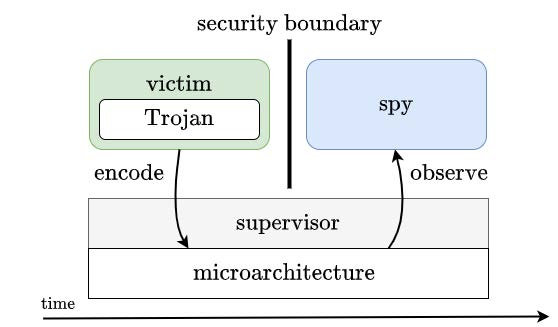
\includegraphics[width=0.7\textwidth]{figure/translation/Figure1.jpg}
    \caption{一种微架构隐蔽通道。受害者进程中的木马将秘密编码进微架构状态。间谍进程通过直接观察微架构状态，或者时间差来推断秘密。}
    \label{fig:convertchannel}
\end{figure}


我们的主要技术贡献如下：
\ding{172} 一种模块化的 FPV 方法，能够穷尽搜索受害者进程中会导致间谍进程可观测执行差异的执行轨迹。
\ding{173}  一套自动化过程，用于生成应用上述方法的 FPV 测试平台，无需任何前期用户输入或 RTL 细节。
\ding{174}  在成熟的开源 RISC-V CVA6 处理器和 MAPLE 加速器中发现了隐蔽信道和硬件缺陷。


我们评估并证明了 AutoCC 具备以下能力：
\ding{172} 在数分钟内触发已知的问题和新的硬件问题（而不是依赖数小时的压力测试仿真）。
\ding{173} 由于执行轨迹长度很短，可以以很少的工作量找到漏洞的成因。
\ding{174} 发现了在实验上可行的隐蔽信道，并且我们能够在 RTL 仿真中验证它们。
\ding{175} 验证了用于修复隐蔽信道的 RTL 改动是有效的，修改后的 RTL 不再产生反例。


\section{背景与先前工作}
进程隔离是系统安全的基础，也是将信息限制在恰当权限域中的主要机制。
隐蔽信道是一种非法的信息流；
它允许跨越操作系统（OS）的安全边界以及本应相互隔离的域发生信息泄露，从而违反系统的安全策略。
例如，一个间谍进程可能利用隐蔽信道从受害者进程中提取秘密。

隐蔽信道可以按照其数据泄漏来源进行分类。
例如，物理信道依赖可测量的电磁场变化或功耗变化来提取信息。
微架构信道则利用对指令集体系结构（ISA）不可见的硬件状态来实现非法信息流。
我们的工作关注的是后者；
在本文剩余部分中，当我们说“隐蔽信道”时，特指微架构隐蔽信道。

\subsection{隐蔽信道}

现有的工作利用 L1-D 缓存、L1-I 缓存、末级缓存（LLC）、TLB、分支预测器以及互连来产生隐蔽信道。
Spectre 攻击 通过将隐蔽信道与推测执行结合，展示了隐蔽信道在瞬态执行攻击中的实用性。
随后又有其他工作通过利用其他隐蔽信道提出了类似攻击。

为了引出威胁场景，假设存在图 \ref{fig:convertchannel} 所示的威胁模型。受害者和间谍是两个在共享硬件上并发运行的应用程序。
它们（理论上）由操作系统使用一种内存保护机制进行隔离。
然而，这条安全边界可以利用隐蔽信道绕过，例如对 L1 数据缓存实施一次 Prime-and-Probe 攻击：
间谍首先通过访问一个大小与数据缓存相同的数据数组中的每个元素（prime buffer），来“填充”数据缓存，使 L1 数据缓存被该数组占满。
在受害者的执行时间片内，恶意的或无意的木马会将秘密 S 编码进微架构状态中；
在这个例子里，它通过用自己的数据逐出 S 对应的缓存行来实现。
最后，间谍再次访问自己的整个 prime buffer，并测量其执行时间。
这样一来，它就能观察到一个与缓存未命中次数线性相关的延迟，并由此推断出木马逐出了多少条缓存行，进而推断出受害者的秘密 S。

资源共享： 当间谍进程与受害者进程共享某种资源时，就可能产生微架构隐蔽信道。
可利用的资源是那些与执行历史有关的状态，并且这些状态会影响未来指令时序或行为的资源。
这不仅包括前面提到的那些硬件单元，也包括仲裁器、缓冲区和有限状态机（FSM）等较为隐蔽的部件。
关于进程如何共享这些资源，我们区分为：
硬件线程同时共享某个资源（例如流水线或共享缓存），以及软件线程对某个资源进行时分共享（例如对一个处理器核或加速器进行时间复用）。
我们的威胁模型（详见第 3.1 节）基于时分共享硬件，因为（a）这在专用硬件中很常见；
并且（b）某个安全域倾向于不同时共享那些受容量或带宽限制的资源（例如指令缓存、TLB、预测器等），以避免由争用引起的信息泄漏。

间谍的观测模型： 为了让数据从受害者进程泄露到间谍进程，间谍必须能够观察到受害者执行的某些信息。
时序信道源于间谍执行中可观测到的时序差异，这些差异由受害者的秘密信息所产生。
其他一些信道则可能基于执行未授权操作的结果，直接推断出这些状态的内容。
后者在安全文献中往往被视为硬件缺陷，因为未授权的访问尝试不应留下与所请求数据相关的痕迹。
正如第 3 节所说明的，AutoCC 在 RTL 模块接口处检测差异，因此它的观测模型适用于所有微架构信道。

受害者的意图：侧信道通常被视为隐蔽信道的一个子集：在侧信道中，受害者进程是无意泄露的;
而其余情况则依赖某个恶意功能，即木马，以某种特定方式使用秘密，从而主动跨越安全边界泄露信息。
我们的方法不关注受害者的意图是什么，它会探索所有可能使隐蔽信道成立的输入。

防护： 现有的工作为时序信道提供了两类替代性防护：硬件资源分区，以及密码软件的常量时间实现。
在多线程处理器中，硬件分区会在空间上划分诸如缓存或预测表等共享资源。
在时分共享处理器中，共享资源则通过一次 flush 在时间上进行分区，这正是我们在本文中评估的机制。
常量时间编程并不必然意味着执行时间是确定的，而是意味着它不依赖于秘密数据。
这种编程风格避免基于秘密数据进行分支和数组索引，其目的在于让善意软件不会作为合法操作的副作用而无意泄露信息（即侧信道）。
默认情况下，我们的方法并不限制可执行的指令类型，因为我们的重点是找到需要在硬件中关闭的隐蔽信道。不过，用户也可以约束 AutoCC 生成的 FPV 环境，只探索符合恒定时间编程规则的执行。
这样的环境将验证某个硬件设计在执行恒定时间软件时是否会泄露数据。
第 5 节将进一步讨论“在硬件中防御隐蔽信道”与“限制软件行为”之间的权衡。

检测： 自 2010 年代初以来，硬件中的信息流安全就一直是活跃研究方向。
这些方案通过硬件组件监控和控制敏感数据流，从而减轻安全威胁，但是这些工作大多通过 RTL 仿真来实现。
因此，它们的有效性取决于所提供的测试用例.
尽管可以使用约束随机测试和模糊测试来生成大量测试用例 ，但它们并不像形式化方法那样能够穷尽探索空间。
细微的时序差异就可能被用来提取秘密。如果目标选择高效，即便是一个二值信道，在 1kHz 上下文切换频率下也能在不到一秒的时间里泄露一个 256 位 AES 密钥。
因此，形式化方法对于发现隐蔽信道至关重要。

\subsection{用于硬件验证的形式化方法}
最早通过形式化验证来保证 RTL 正确性的工作，采用了结合 SAT 求解器和二叉判定图（BDD）的模型检测方法。
对于给定的被测设计（DUT），模型检测器会在其输入以及指定假设的条件下，生成 DUT 所有可能执行构成的状态空间。
假设通过禁止某些行为来约束状态空间探索，而断言则检查这些被探索路径上的性质是否全部成立。
FPV 后端工具会使用各种不同的求解引擎 来穷尽搜索属性违例（反例）。
有界模型检测（BMC）是当今许多求解引擎的首选方法。
在 BMC 中，正确性属性会被展开到一个有界的转移步数 $k$，从而将模型检测问题归约为一个 SAT 实例.
对于 AutoCC 来说，这意味着要证明该属性对 DUT 的所有长度为 $k$ 个周期的执行都成立——每次成功证明之后，$k$ 都会递增。
这对完备性意味着什么？对某个属性完成一个 $k$ 周期的有界证明，意味着该属性对长度小于或等于 $k$ 个周期的执行成立——更长的执行仍然可能导致属性违例。
要对无界执行证明该属性，$k$ 必须达到一个完备性阈值。
一个朴素的阈值是模型中的状态数；更紧的阈值则是模型中最远两个状态之间的最短路径长度。
在实践中，达到这个完备性阈值并不总是可行；检测器可能会耗尽时间或内存，或者该阈值本身就很难计算。

已有工作已经将 FPV 应用到不同的方面上：RTLCheck 用于根据内存一致性模型验证 CPU 的 RTL 实现；
ILA 根据其功能规范生成设计的 Verilog 模型，并将其与 RTL 实现进行比较；
AutoSVA 检查 RTL 模块交互的活性性质。
活性性质规定“某件好事最终会发生”，例如一个请求最终会得到应答；
而安全性质则规定“某件坏事绝不会发生”，例如某个响应必须先有一个请求。
在隐蔽信道的场景下，我们关注的是能够检测跨进程数据泄露的安全性质。
第 3 节将详细说明 AutoCC 如何将这种检测表述为一个 FPV 问题。

形式化方法也已被用于检测安全漏洞。
InSpectre 建立处理器的形式模型，以检测将推测执行与隐蔽信道结合的 Spectre 类攻击.
UPEC 使用 FPV 来检测由于未授权操作副作用所导致的内存泄漏。
然而，UPEC 仅限于发现内存泄漏（例如通过陈旧的微架构状态），并不考虑由于执行时间导致的泄漏。

为了扩展基于形式化方法的先前工作范围，AutoCC 在硬件 RTL 上使用 FPV，自动检测那些源自某种状态的微架构隐蔽信道;
该状态的取值依赖于先前执行，并且会影响未来指令的时序。
AutoCC 补充了诸如 Channel Bench这样的经验型隐蔽信道测量框架；
这类框架能够展示某些特定信道的存在或不存在，但不能覆盖全部信道。

\section{AutoCC 方法}
本节首先给出本文所应对的威胁模型，即进程在共享硬件上进行时间复用执行的场景。
接着，第 3.2 节说明我们如何将该威胁模型形式化（变成 FPV 引擎能够求解的问题），以便自动发现这些进程之间的隐蔽信道。
第 3.3 节解释如何利用我们的自动化流程将该方法应用到一个 RTL 项目上，该流程会生成 FPV 测试平台和工具绑定。
第 3.4 节提出了一条通过模块化将 AutoCC 应用于大型项目的可行路径。
最后，第 3.5 节介绍了两种利用 AutoCC 来辅助正确设计防御隐蔽信道的时间型防护机制的策略。

\subsection{AutoCC 的威胁模型}

AutoCC 的威胁模型假设存在两个进程：攻击者进程和受害者进程。
它们在时分共享硬件上执行，并通过由操作系统（OS）强制执行的一次上下文切换来彼此分隔。
这两个进程都不可信，而受害者运行在一个受控环境中，OS 会限制受害者能够与谁通信。
攻击者进程不具备任何特殊权限，并在属于自己的安全域中执行。
按理说，由于这两个进程位于不同的安全域中，因此任何硬件状态都不应将数据从受害者泄露给攻击者。
然而，攻击者可能利用隐蔽信道非法提取信息。
它最主要的工具是一段木马代码，即受害者进程中的一段代码，它使数据泄漏成为可能（如图 \ref{fig:convertchannel} 所示）。

作为面向硬件设计人员的工具，AutoCC 强调的是敏感性。
也就是说，它的目标是向设计人员暴露全部可能的隐蔽信道，然后由设计人员决定采取何种措施（第 5 节将讨论相关权衡）。
因此，我们不对秘密数据如何被编码进已被攻陷的硬件状态施加任何约束，即木马既可以是受害者进程中隐藏的恶意功能，也可以是某段无害代码，它作为合法操作的副作用无意地泄露数据。
以发现每一个隐蔽信道——不论使其成立的代码有无恶意意图——为目标，使我们能够证明更强的正确性断言，即：没有隐蔽信道的硬件，也必然没有侧信道。

我们进一步指出，这一威胁模型并不限于 CPU。
加速器和其他专用硬件模块往往也是在进程之间以时间复用的方式共享的，它们同样容易受到隐蔽信道影响。
这些专用硬件模块所能执行的操作，可以被视为它们的 ISA。
在本文剩余部分中，“被测设计”（DUT）指我们正在测试的顶层模块，无论它的专用化程度如何。

\subsection{将威胁模型形式化为 FPV 问题}

在定义完威胁模型之后，我们现在说明如何将它形式化为一个 FPV 问题：通过一步步让 FPV 工具越来越接近对上述场景的建模。
在我们的形式化中，采用如下定义：

\textbf{定义 1（状态）}: DUT 的状态，是该硬件模块及其所实例化子模块中所有触发器、寄存器和存储单元的集合。
DUT 定义了求解的边界；位于 DUT 之外的任何 RTL 都不在考虑之列。这一区分对我们在第 3.4 节中关于模块化的讨论尤其重要。

\textbf{定义 2（架构状态）}。 DUT 的架构状态（$arch$）是其状态中能够通过 ISA 指令读取到的那一部分。

\textbf{定义 3（微架构状态）}。 微架构状态（$\mu arch$）是状态中不属于 $arch$ 的那一部分（即不能通过 ISA 指令直接读取的部分）。

在 DUT 上执行的某个进程自然会改变 $arch$ 和 $\mu arch$ 的取值。
因此，这些状态的隔离（相对于它们所属的进程而言）是软件与硬件的共同责任。
一个正确实现的 OS 会：（1）保护那些只能通过特权模式访问的 $arch$；
以及（2）在另一个进程开始之前交换 $arch$ 的取值。
一个设计良好且安全的硬件，要么会对任何可能将数据从一个进程泄露给另一个进程的 $\mu arch$ 进行分区，要么会将其 flush。
按照这些定义，AutoCC 假设 OS 是正确的，并检查 $\mu arch$ 的隔离性。

数据泄漏： 数据泄漏的发生必须满足两个条件。
第一，在间谍进程开始时，$\mu arch$ 的取值由受害者进程的行为决定。
也就是说，基于受害者数据的不同取值，至少存在两种受害者进程执行，它们会导致 $\mu arch$ 的不同取值。
第二，存在同一个间谍程序的至少两种执行，它们从相同的 $arch$ 值出发，却仅仅由于 $\mu arch$ 的差异而导向不同的 $arch$。
我们的目标是建立一个环境，使 FPV 工具能够探索受害者进程和间谍进程的一切可能执行。

AutoCC 通过如下方式设置 DUT 的两个实例——宇宙 $\alpha$ 和 $\beta$——来实现这一点（同时参见图 \ref{fig:overview}）：两个宇宙都从同一个复位状态开始；
每个宇宙都有自己的一组输入和输出信号;
由于每组输入信号都由 FPV 工具分别驱动，因此每个宇宙都可以采取任意合法执行。

\begin{figure}
    \centering
    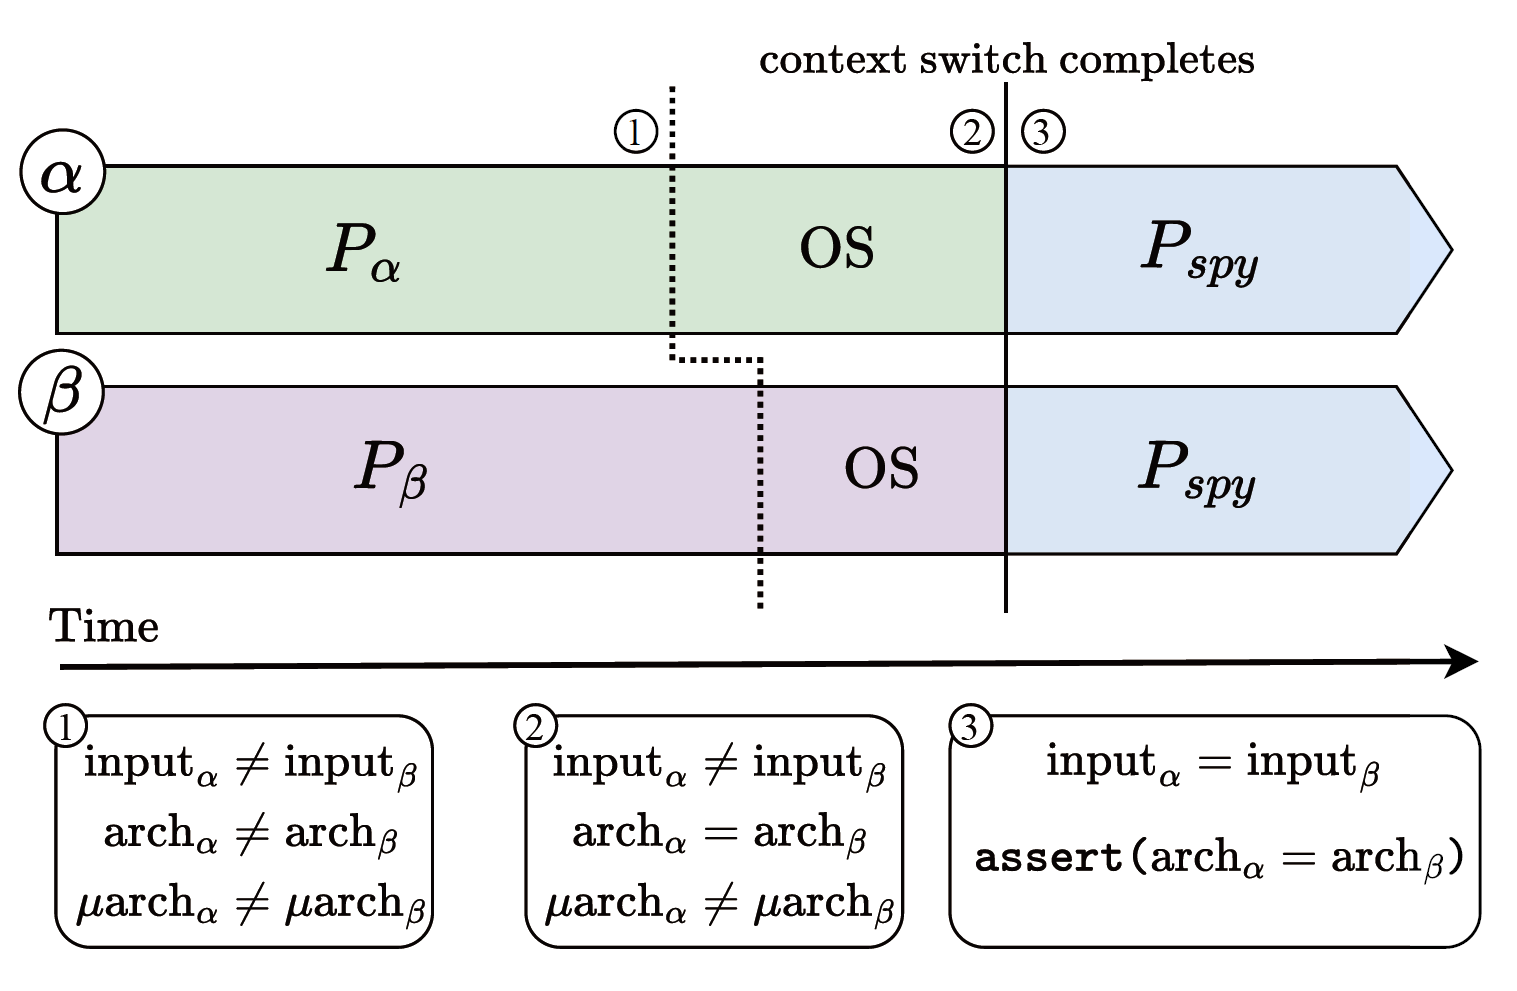
\includegraphics[width=0.85\textwidth]{figure/translation/Figure2.png}
    \caption{AutoCC 总览}
    \label{fig:overview}
\end{figure}


图 \ref{fig:overview} 还定义了 DUT 执行期间发生的三个事件。
第一个事件是受害者进程结束（以及上下文切换开始）的时刻，此时 $\alpha$ 和 $\beta$ 可以处于任意可达状态，这些状态是它们在任意多个周期之后的结果。
这些状态代表受害者进程的一切可能执行。
尽管上下文切换的开始时刻可以错开，但其结束时刻充当了 $\alpha$ 与 $\beta$ 之间的同步点，迫使这两个此前执行不同的宇宙走向收敛。
要实现这一点，上下文切换必须确保：在其完成时，（1）$arch_{\alpha}$ 和 $arch_{\beta}$ 完全相同，并且（2）如果存在微架构 flush 机制，那么该机制已经执行完毕。
在满足这两个条件后，假定 $\alpha$ 和 $\beta$ 现在都在执行同一个进程，即刚刚被切入的间谍进程。

两个宇宙的输入随后被强制为相等，以确保任何被观察到的分歧都只能来自 $\mu arch_{\alpha}$ 与 $\mu arch_{\beta}$ 的不同取值。
在这个上下文切换之后的世界里，我们断言：在每一个周期中，$arch_{\alpha}$ 与 $arch_{\beta}$ 都必须相等。

如果这个断言被违反，意味着什么？
对这一断言的一个反例（CEX）意味着：
在切换之后的某个周期，$\alpha$ 和 $\beta$ 发生了精确到周期级的分歧，并且这种差异是由它们在切换之前的执行不同的指令所导致的。
换句话说，存在一种机制，使受害者进程中的某段代码能够影响间谍进程的执行，即存在一个隐蔽信道。
分析该反例并找出这种分歧的根源，就能揭示该信道是如何工作的；
我们将在第 4 节展示这种编码与观测是如何发生的。

\begingroup
    \linespreadsingle{}
    \printbibliography[title={外文翻译参考文献}]
\endgroup
